\documentclass[english, 11 pt, class=article, crop=false]{standalone}
\usepackage[T1]{fontenc}
%\renewcommand*\familydefault{\sfdefault} % For dyslexia-friendly text
\usepackage{lmodern} % load a font with all the characters
\usepackage{geometry}
\geometry{verbose,paperwidth=16.1 cm, paperheight=24 cm, inner=2.3cm, outer=1.8 cm, bmargin=2cm, tmargin=1.8cm}
\setlength{\parindent}{0bp}
\usepackage{import}
\usepackage[subpreambles=false]{standalone}
\usepackage{amsmath}
\usepackage{amssymb}
\usepackage{esint}
\usepackage{babel}
\usepackage{tabu}
\makeatother
\makeatletter

\usepackage{titlesec}
\usepackage{ragged2e}
\RaggedRight
\raggedbottom
\frenchspacing

% Norwegian names of figures, chapters, parts and content
\addto\captionsenglish{\renewcommand{\figurename}{Figur}}
\makeatletter
\addto\captionsenglish{\renewcommand{\chaptername}{Kapittel}}
\addto\captionsenglish{\renewcommand{\partname}{Del}}


\usepackage{graphicx}
\usepackage{float}
\usepackage{subfig}
\usepackage{placeins}
\usepackage{cancel}
\usepackage{framed}
\usepackage{wrapfig}
\usepackage[subfigure]{tocloft}
\usepackage[font=footnotesize,labelfont=sl]{caption} % Figure caption
\usepackage{bm}
\usepackage[dvipsnames, table]{xcolor}
\definecolor{shadecolor}{rgb}{0.105469, 0.613281, 1}
\colorlet{shadecolor}{Emerald!15} 
\usepackage{icomma}
\makeatother
\usepackage[many]{tcolorbox}
\usepackage{multicol}
\usepackage{stackengine}

\usepackage{esvect} %For vectors with capital letters

% For tabular
\usepackage{array}
\usepackage{multirow}
\usepackage{longtable} %breakable table

% Ligningsreferanser
\usepackage{mathtools}
\mathtoolsset{showonlyrefs}

% index
\usepackage{imakeidx}
\makeindex[title=Indeks]

%Footnote:
\usepackage[bottom, hang, flushmargin]{footmisc}
\usepackage{perpage} 
\MakePerPage{footnote}
\addtolength{\footnotesep}{2mm}
\renewcommand{\thefootnote}{\arabic{footnote}}
\renewcommand\footnoterule{\rule{\linewidth}{0.4pt}}
\renewcommand{\thempfootnote}{\arabic{mpfootnote}}

%colors
\definecolor{c1}{cmyk}{0,0.5,1,0}
\definecolor{c2}{cmyk}{1,0.25,1,0}
\definecolor{n3}{cmyk}{1,0.,1,0}
\definecolor{neg}{cmyk}{1,0.,0.,0}

% Lister med bokstavar
\usepackage[inline]{enumitem}

\newcounter{rg}
\numberwithin{rg}{chapter}
\newcommand{\reg}[2][]{\begin{tcolorbox}[boxrule=0.3 mm,arc=0mm,colback=blue!3] {\refstepcounter{rg}\phantomsection \large \textbf{\therg \;#1} \vspace{5 pt}}\newline #2  \end{tcolorbox}\vspace{-5pt}}

\newcommand\alg[1]{\begin{align} #1 \end{align}}

\newcommand\eks[2][]{\begin{tcolorbox}[boxrule=0.3 mm,arc=0mm,enhanced jigsaw,breakable,colback=green!3] {\large \textbf{Eksempel #1} \vspace{5 pt}\\} #2 \end{tcolorbox}\vspace{-5pt} }

\newcommand{\st}[1]{\begin{tcolorbox}[boxrule=0.0 mm,arc=0mm,enhanced jigsaw,breakable,colback=yellow!12]{ #1} \end{tcolorbox}}

\newcommand{\spr}[1]{\begin{tcolorbox}[boxrule=0.3 mm,arc=0mm,enhanced jigsaw,breakable,colback=yellow!7] {\large \textbf{Språkboksen} \vspace{5 pt}\\} #1 \end{tcolorbox}\vspace{-5pt} }

\newcommand{\sym}[1]{\colorbox{blue!15}{#1}}

\newcommand{\info}[2]{\begin{tcolorbox}[boxrule=0.3 mm,arc=0mm,enhanced jigsaw,breakable,colback=cyan!6] {\large \textbf{#1} \vspace{5 pt}\\} #2 \end{tcolorbox}\vspace{-5pt} }

\newcommand\algv[1]{\vspace{-11 pt}\begin{align*} #1 \end{align*}}

\newcommand{\regv}{\vspace{5pt}}
\newcommand{\mer}{\textsl{Merk}: }
\newcommand{\mers}[1]{{\footnotesize \mer #1}}
\newcommand\vsk{\vspace{11pt}}
\newcommand\vs{\vspace{-11pt}}
\newcommand\vsb{\vspace{-16pt}}
\newcommand\sv{\vsk \textbf{Svar} \vspace{4 pt}\\}
\newcommand\br{\\[5 pt]}
\newcommand{\figp}[1]{../fig/#1}
\newcommand\algvv[1]{\vs\vs\begin{align*} #1 \end{align*}}
\newcommand{\y}[1]{$ {#1} $}
\newcommand{\os}{\\[5 pt]}
\newcommand{\prbxl}[2]{
\parbox[l][][l]{#1\linewidth}{#2
	}}
\newcommand{\prbxr}[2]{\parbox[r][][l]{#1\linewidth}{
		\setlength{\abovedisplayskip}{5pt}
		\setlength{\belowdisplayskip}{5pt}	
		\setlength{\abovedisplayshortskip}{0pt}
		\setlength{\belowdisplayshortskip}{0pt} 
		\begin{shaded}
			\footnotesize	#2 \end{shaded}}}

\renewcommand{\cfttoctitlefont}{\Large\bfseries}
\setlength{\cftaftertoctitleskip}{0 pt}
\setlength{\cftbeforetoctitleskip}{0 pt}

\newcommand{\bs}{\\[3pt]}
\newcommand{\vn}{\\[6pt]}
\newcommand{\fig}[1]{\begin{figure}
		\centering
		\includegraphics[]{\figp{#1}}
\end{figure}}

\newcommand{\figc}[2]{\begin{figure}
		\centering
		\includegraphics[]{\figp{#1}}
		\caption{#2}
\end{figure}}

\newcommand{\sectionbreak}{\clearpage} % New page on each section

\newcommand{\nn}[1]{
\begin{equation}
	#1
\end{equation}
}

% Equation comments
\newcommand{\cm}[1]{\llap{\color{blue} #1}}

\newcommand\fork[2]{\begin{tcolorbox}[boxrule=0.3 mm,arc=0mm,enhanced jigsaw,breakable,colback=yellow!7] {\large \textbf{#1 (forklaring)} \vspace{5 pt}\\} #2 \end{tcolorbox}\vspace{-5pt} }
 
%colors
\newcommand{\colr}[1]{{\color{red} #1}}
\newcommand{\colb}[1]{{\color{blue} #1}}
\newcommand{\colo}[1]{{\color{orange} #1}}
\newcommand{\colc}[1]{{\color{cyan} #1}}
\definecolor{projectgreen}{cmyk}{100,0,100,0}
\newcommand{\colg}[1]{{\color{projectgreen} #1}}

% Methods
\newcommand{\metode}[2]{
	\textsl{#1} \\[-8pt]
	\rule{#2}{0.75pt}
}

%Opg
\newcommand{\abc}[1]{
	\begin{enumerate}[label=\alph*),leftmargin=18pt]
		#1
	\end{enumerate}
}
\newcommand{\abcs}[2]{
	\begin{enumerate}[label=\alph*),start=#1,leftmargin=18pt]
		#2
	\end{enumerate}
}
\newcommand{\abcn}[1]{
	\begin{enumerate}[label=\arabic*),leftmargin=18pt]
		#1
	\end{enumerate}
}
\newcommand{\abch}[1]{
	\hspace{-2pt}	\begin{enumerate*}[label=\alph*), itemjoin=\hspace{1cm}]
		#1
	\end{enumerate*}
}
\newcommand{\abchs}[2]{
	\hspace{-2pt}	\begin{enumerate*}[label=\alph*), itemjoin=\hspace{1cm}, start=#1]
		#2
	\end{enumerate*}
}

% Oppgaver
\newcommand{\opgt}{\phantomsection \addcontentsline{toc}{section}{Oppgaver} \section*{Oppgaver for kapittel \thechapter}\vs \setcounter{section}{1}}
\newcounter{opg}
\numberwithin{opg}{section}
\newcommand{\op}[1]{\vspace{15pt} \refstepcounter{opg}\large \textbf{\color{blue}\theopg} \vspace{2 pt} \label{#1} \\}
\newcommand{\ekspop}[1]{\vsk\textbf{Gruble \thechapter.#1}\vspace{2 pt} \\}
\newcommand{\nes}{\stepcounter{section}
	\setcounter{opg}{0}}
\newcommand{\opr}[1]{\vspace{3pt}\textbf{\ref{#1}}}
\newcommand{\oeks}[1]{\begin{tcolorbox}[boxrule=0.3 mm,arc=0mm,colback=white]
		\textit{Eksempel: } #1	  
\end{tcolorbox}}
\newcommand\opgeks[2][]{\begin{tcolorbox}[boxrule=0.1 mm,arc=0mm,enhanced jigsaw,breakable,colback=white] {\footnotesize \textbf{Eksempel #1} \\} \footnotesize #2 \end{tcolorbox}\vspace{-5pt} }
\newcommand{\rknut}{
Rekn ut.
}

%License
\newcommand{\lic}{\textit{Matematikken sine byggesteinar by Sindre Sogge Heggen is licensed under CC BY-NC-SA 4.0. To view a copy of this license, visit\\ 
		\net{http://creativecommons.org/licenses/by-nc-sa/4.0/}{http://creativecommons.org/licenses/by-nc-sa/4.0/}}}

%referances
\newcommand{\net}[2]{{\color{blue}\href{#1}{#2}}}
\newcommand{\hrs}[2]{\hyperref[#1]{\color{blue}\textsl{#2 \ref*{#1}}}}
\newcommand{\rref}[1]{\hrs{#1}{regel}}
\newcommand{\refkap}[1]{\hrs{#1}{kapittel}}
\newcommand{\refsec}[1]{\hrs{#1}{seksjon}}

\newcommand{\mb}{\net{https://sindrsh.github.io/FirstPrinciplesOfMath/}{MB}}


%line to seperate examples
\newcommand{\linje}{\rule{\linewidth}{1pt} }

\usepackage{datetime2}
%%\usepackage{sansmathfonts} for dyslexia-friendly math
\usepackage[]{hyperref}


\newcommand{\note}{Merk}
\newcommand{\notesm}[1]{{\footnotesize \textsl{\note:} #1}}
\newcommand{\ekstitle}{Eksempel }
\newcommand{\sprtitle}{Språkboksen}
\newcommand{\expl}{forklaring}

\newcommand{\vedlegg}[1]{\refstepcounter{vedl}\section*{Vedlegg \thevedl: #1}  \setcounter{vedleq}{0}}

\newcommand\sv{\vsk \textbf{Svar} \vspace{4 pt}\\}

%references
\newcommand{\reftab}[1]{\hrs{#1}{tabell}}
\newcommand{\rref}[1]{\hrs{#1}{regel}}
\newcommand{\dref}[1]{\hrs{#1}{definisjon}}
\newcommand{\refkap}[1]{\hrs{#1}{kapittel}}
\newcommand{\refsec}[1]{\hrs{#1}{seksjon}}
\newcommand{\refdsec}[1]{\hrs{#1}{delseksjon}}
\newcommand{\refved}[1]{\hrs{#1}{vedlegg}}
\newcommand{\eksref}[1]{\textsl{#1}}
\newcommand\fref[2][]{\hyperref[#2]{\textsl{figur \ref*{#2}#1}}}
\newcommand{\refop}[1]{{\color{blue}Oppgave \ref{#1}}}
\newcommand{\refops}[1]{{\color{blue}oppgave \ref{#1}}}
\newcommand{\refgrubs}[1]{{\color{blue}gruble \ref{#1}}}

\newcommand{\openmathser}{\openmath\,-\,serien}

% Exercises
\newcommand{\opgt}{\newpage \phantomsection \addcontentsline{toc}{section}{Oppgaver} \section*{Oppgaver for kapittel \thechapter}\vs \setcounter{section}{1}}


% Sequences and series
\newcommand{\sumarrek}{Summen av en aritmetisk rekke}
\newcommand{\sumgerek}{Summen av en geometrisk rekke}
\newcommand{\regnregsum}{Regneregler for summetegnet}

% Trigonometry
\newcommand{\sincoskomb}{Sinus og cosinus kombinert}
\newcommand{\cosfunk}{Cosinusfunksjonen}
\newcommand{\trid}{Trigonometriske identiteter}
\newcommand{\deravtri}{Den deriverte av de trigonometriske funksjonene}
% Solutions manual
\newcommand{\selos}{Se løsningsforslag.}
\newcommand{\se}[1]{Se eksempel på side \pageref{#1}}

%Vectors
\newcommand{\parvek}{Parallelle vektorer}
\newcommand{\vekpro}{Vektorproduktet}
\newcommand{\vekproarvol}{Vektorproduktet som areal og volum}


% 3D geometries
\newcommand{\linrom}{Linje i rommet}
\newcommand{\avstplnpkt}{Avstand mellom punkt og plan}


% Integral
\newcommand{\bestminten}{Bestemt integral I}
\newcommand{\anfundteo}{Analysens fundamentalteorem}
\newcommand{\intuf}{Integralet av utvalge funksjoner}
\newcommand{\bytvar}{Bytte av variabel}
\newcommand{\intvol}{Integral som volum}
\newcommand{\andordlindif}{Andre ordens lineære differensialligninger}



\begin{document}
\section{Vektorer i rommet}\index{vektor!i rommet}
I \tmen\ har vi sett på todimensjonale vektorer beskrevet ved hjelp av en $ x $- og en $ y $-akse. Når vi skal beskrive en \outl{tredimensjonal vektor}, innfører vi i tillegg en $ z $-akse som står normalt på de to andre aksene. 

\figc{vekt1}{$ \vec{u}=[2, 3, 4] $\label{vekt1}}

\regdef[Vektoren mellom to punkt \index{vektor!mellom to punkt}]{
	En vektor $ \vec{v} $ med startpunkt $ {A=(x_1, y_1, z_1)}$ og endepunkt ${B=(x_2, y_2, z_2) }$ er gitt som
	\begin{equation}\label{vektmpunkt}
		\vec{u}= [x_2-x_1, y_2-y_1, z_2-z_1] 
	\end{equation} \vs
} 
\eks{
	Finn vektoren $ \vec{u} $ mellom punktet  ${A=(1, 2, 0) } $ og $ B=(3, 0,\\ 1) $.
	
	\sv \vs
	\algv{
		\vec{u} &= [3-1, 0-2, 1-0] \\
		& = [2, -2, 1]	}\vs
} \vsk
\newpage
\info{Merk}{
Seksjon \ref{vekleng}\,-\,\ref{vinkrogpar} handler om visse egenskaper og regneregler for tredimensjonale vektorer. Det er mange likheter ved todimensjonale og tredimensjonale vektorer, så i tilfeller hvor en regel mangler forklaring, er det fordi forklaringen for det todimensjonale tilfellet (som du finner i \tmen) enkelt kan generaliseres til det tredimensjonale tilfellet.
}

\section{Lengden til en vektor \label{vekleng}}\index{vektor!lengden til}
La oss prøve å finne lengden til en vektor $ {\vec{u}=[x_1, y_1, z_1]} $, som skissert i \fref{lenu}. Grafisk er lengden avstanden fra den butte enden til pilspissen.
\figc{vekt3}{\label{lenu}}
Vi kan alltid lage en rettvinklet trekant med sidelengder $ |\vec{u}| $, $ z_1 $ og $ \hat{u}=\sqrt{x_1^2+y_1^2} $. Av Pytagoras' setning har vi da at
\alg{
	|\vec{u}|&=\sqrt{\hat{u}^2+z_1^2} \\
	&= \sqrt{x_1^2+y_1^2+z_1^2} 
}
\reg[lengden til en vektor]{
	Lengden $ |\vec{u}|$ av en vektor $ {\vec{u}=[x_1, y_1, z_1]} $ er gitt som
	\nreq{|\vec{u}|=\sqrt{x_1^2+y_1^2+z_1^2} \label{lengd}} \vs
}
\eks{
	Finn lengden til vektoren $ {\vec{u}=[-2, 4, 1]} $.
	
	\sv \vs
	\algv{
		|\vec{u}|&= \sqrt{(-2)^2+4^2+1^2} \\
		&= \sqrt{4+16+1} \\
		&= \sqrt{21}
	}\vs \vspace{-4pt}
}
\eks[2]{
	Finn lengden til vektoren ${\vec{a}= [-9, 18, 27]} $.
	
	\sv
	Ved å bruke \eqref{fellesfakt} sparer vi oss for kvadrater av store tall:
	\[ [-9, 18, 27]=9[-1, 2, 3] \]
	Lengden blir da (se \refops{lenfakt})
	\alg{
		|\vec{a}|&= 9\sqrt{(-1)^2+2^2+3^2} \\
		&= 9\sqrt{14}
	}\vs
}

\section{Regneregler og skalarprodukt}
\reg[Regneregler for vektorer]{
	Gitt vektorene $ {\vec{u}=[x_1, y_1, z_1]} $ og $ {\vec{v}=[x_2, y_2, z_2]} $, punktet ${ A=(x_0,y_0,z_0)} $ og en konstant $ t $. Da er
	\begin{align}
		A+\vec{u} &= (x_0+x_1, y_0+y_1, z_0+z_1) \label{punktplvektor}	\\
		\vec{u}+\vec{v} &= [x_1+x_2, y_1+y_2, z_1+z_2] \\
		\vec{u}-\vec{v} &= [x_1-x_2, y_1-y_2, z_1-z_2] 
	\end{align}
	Summen eller differansen av $ \vec{u} $ og $ \vec{v} $ kan vi tegne slik:
	\begin{figure}
		\centering
		\subfloat{\includegraphics[scale=1]{\figp{uplusv}}}\qquad\quad
		\subfloat{\includegraphics[scale=1]{\figp{uminusv}}}
	\end{figure}\vs
} \regv

\reg[Regneregler for vektorer]{
	For vektorene $\vec{u}$, $ \vec{v} $ og $\vec{w} $, og et tall $ t $, har vi at
	\begin{align}
		t\vec{u} &= [tx_1, ty_1, tz_1] \label{fellesfakt} \br
		t(\vec{u}+\vec{v})&= t\vec{u}+t\vec{v}\br
		(\vec{u}+\vec{v})+\vec{w} &= \vec{u}+(\vec{v}+\vec{w}) \br
		\vec{u}-(\vec{v}+\vec{w}) &= \vec{u}-\vec{v}-\vec{w}
	\end{align}
}
\newpage
\eks[]{
	Et parallellogram er tegnet inn i figuren under.
	\begin{figure}
		\centering
		\includegraphics[]{\figp{par2}}
	\end{figure}
	Vis at midpunktet $ M $ til diagonalen $ AG $ også er midtpunktet til diagonalen $ CE $. \\
	
	\sv
	Vektoren $ \vv{AG} $ er gitt som
	\[ \vv{AG}= \vec{a}+\vec{b}+\vec{c} \]
	Dette betyr at
	\alg{
		\vv{AM}&= \frac{1}{2}\vv{AG} \\
		&= \frac{1}{2}(\vec{a}+\vec{b}+\vec{c}) 	
	}
	Vi kaller midpunktet til $ CE $ for $ M_1 $. Da har vi at
	\alg{
		\vv{CM_1} &= \frac{1}{2}\vv{CE}\\
		&= \frac{1}{2}(\vec{c}-\vec{a}-\vec{b})
	}
	Videre er
	\alg{
		\vv{AM_1}&=\vec{a}+\vec{b}+\vv{CM_1} \\
		&= \vec{a}+\vec{b}+ \frac{1}{2}(\vec{c}-\vec{a}-\vec{b})\\
		&= \frac{1}{2}(\vec{a}+\vec{b}+\vec{c}) \\
		&= \vv{AM}
	}
	Dette må bety at $ M=M_1 $.
}

\reg[Skalarproduktet I]{
	Skalarproduktet av to vektorer  $ {\vec{u}=[x_1, y_1, z_1]} $ og $ {\vec{v}=[x_2, y_2, z_2]} $ kan skrives som	
	\begin{equation}
		\vec{u} \cdot \vec{v} = x_1 x_2+y_1 y_2+z_1 z_2
	\end{equation}
	
	For særtilfellet $ \vec{u}\cdot\vec{u} $ er
	\begin{equation}
		\vec{u}\cdot\vec{u}=\vec{u}^{\,2}
	\end{equation}	\vs
	
}
\eks{Finn skalarproduktet av vektorene $ {\vec{a}=[1, 2, 3]} $ og $ \vec{b}=[4,-3,\\-2] $.
	
	\sv \vs
	\algv{\vec{a}\cdot\vec{b}&= 1\cdot4 + 2\cdot(-3)+3\cdot(-2)\\ &=-8 }\vs
} \vsk

\reg[Skalarproduktet II]{
	Skalarproduktet av to vektorer  $ \vec{u} $ og $ \vec{v}$ er gitt som
	\begin{equation}
		\vec{u} \cdot \vec{v}= |\vec{u}| |\vec{v}| \cos \theta \label{skal2}
	\end{equation}
	hvor $ \theta=\angle(\vec{u}, \vec{v}) $.
}
\eks[1]{
	En vektor $ \vec{a} $ har lengde 3 og en vektor $ \vec{b} $ har lengde 2. De utspenner vinkelen $ 45^\circ $. Finn skalarproduktet $ \vec{a}\cdot\vec{b}$. \\
	
	\sv
	\vs
	\vs
	\algv{\vec{a}\cdot\vec{b} &= 3\cdot2 \cos (45^\circ) \br
		&= 6\cdot\frac{\sqrt{2}}{2} \br
		&= 3\sqrt{2}}\vs
}
\newpage
\eks[2]{
	Finn vinkelen $ v$ utspent av vektorene $ {\vec{a}=[-5, 4, -3]}$ og $ {\vec{b}=[-2, 5, -5]} $. \\
	
	\sv
	Vi starter med å finne lengdene og skalarproduktene av vektorene:
	\alg{
		|\vec{a}|&= \sqrt{(-5)^2+4^2+(-3)^2} \\
		&= \sqrt{50} \\
		&= 5\sqrt{2} \\
		|\vec{b}| &= \sqrt{(-2)^2+5^2+(-5)^2} \\
		&= \sqrt{54} \\
		&= 3\sqrt{6} \\
		\vec{a}\cdot\vec{b} &= (-5)\cdot(-2) + 5\cdot4+(-3)\cdot(-5) \\&= 45
	}
	Videre har vi at
	\algv{\vec{a}\cdot \vec{b}&= |\vec{a}||\vec{b}|\cos v \\
		45 &= 5\sqrt{2}\cdot3\sqrt{6}\cos v \\
		\cos v &= \frac{5\cdot9}{5\cdot3\sqrt{12}} \\
		&= \frac{5\cdot9}{4\cdot3\cdot2\sqrt{3}}  \\
		&= \frac{3}{2\sqrt{3}} \\
		&= \frac{3}{2\sqrt{3}} \cdot \frac{\sqrt{3}}{\sqrt{3}} \\
		&= \frac{\sqrt{3}}{2}
	}
	Siden $ {\cos v = \frac{\sqrt{3}}{2}} $, er $ {v=30^\circ} $.
}
\reg[Regneregler for skalarproduktet]{
	For vektorene $ \vec{u} $, $ \vec{v} $ og $ \vec{w} $ har vi at
	\alg{
		\vec{u}\cdot\vec{v} &= \vec{v}\cdot\vec{u} \\
		\vec{u}\cdot\left(\vec{v}+\vec{w}\right) &= \vec{u}\cdot\vec{v}+\vec{u}\cdot\vec{w} \\
		\left(\vec{u}+\vec{v}\right)^2 &= \vec{u}^{\,2} + 2\vec{u}\cdot\vec{v}+\vec{v}^{\,2}
	}\vs
}
\eks{Forkort uttrykket
	\[   \vec{b}\cdot(\vec{a}+\vec{c}) + \vec{a}\cdot(\vec{a}+\vec{b})+\vec{b}^{\,2} \]
	
	når du vet at $ \vec{b}\cdot\vec{c}=0 $. \\
	
	\sv
	\algv{\vec{b}\cdot(\vec{a}+\vec{c}) + \vec{a}\cdot(\vec{a}+\vec{b})+\vec{b}^{\,2} &= \vec{b}\cdot\vec{a}+\vec{b}\cdot\vec{c} + \vec{a}\cdot\vec{a}+\vec{a}\cdot\vec{b}+\vec{b}^2 \\
		&= \vec{a}^{\,2} + 2 \vec{a}\cdot \vec{b} + \vec{b}^{\,2} \\
		&= \left(\vec{a}+ \vec{b}\right)^2
	}\vs
}

\section{Vinkelrette og parallelle vektorer \label{vinkrogpar}}
\reg[Vinkelrette vektorer ]{
	To vektorer $ \vec{u} $ og $ \vec{v} $ står vinkelrett på hverandre hvis skalarproduktet av dem er null:
	\begin{equation}\label{vnkr}
		\vec{u} \cdot \vec{v} = 0\iff \vec{u}\perp \vec{v}
	\end{equation}
}

\eks[1]{
Sjekk om vektorene $ {\vec{a}=[5, -3, 2]} $ og $ {\vec{b}=[2, 4, 1]} $ er ortogonale.

\sv \vs
\algv{
\vec{a}\cdot\vec{b}&=[5, -3, 2]\cdot[2, 4, 1] \\
&=10-12+2 \\
&=0
}
Altså er $ \vec{a}\perp\vec{b} $.
}\vsk

\reg[\parvek \label{parvek}]{
	To vektorer $ {\vec{u}=[x_1, y_1, z_1]} \text{ og } {\vec{v}=[x_2, y_2, z_2]} $ har vi at
	\begin{equation}
		\frac{x_1}{x_2}=\frac{y_1}{y_2}=\frac{z_1}{z_2} \iff \vec{u}\parallel\vec{v}
	\end{equation}
Alternativt, for et tall $ t $ har vi at
\begin{equation}
	\vec{u}=t\vec{v}\iff \vec{u}\parallel\vec{v}
\end{equation}
}
\newpage
\eks[1]{
	Gitt vektorene $ {\vec{u}=[1, 2, 3] }$ og ${\vec{v}=[3, 2(1-t), 11+t]} $, finn \textit{t} slik at $ \vec{u}$ og $ \vec{v} $ er parallelle.  \\
	
	\sv 
	Vi starter med å kreve at forholdet mellom korresponderende komponenter er likt. Vi dividerer $ x $- og $ y$-komponenten i $ \vec{v} $ med henholdsvis $ x $- og $ y$-komponenten i $ \vec{u} $:
	\begin{align*}
		\frac{3}{1} & = \frac{2(1-t)}{2} \\
		3 & = 1- t \\
		t &= -2
	\end{align*}
	Siden forholdet mellom de to $ x $-komponentene og de to $ y $-koordinatene er 3, må dette også stemme for $ z $-koordinatene for at $ \vec{u} $ og $ \vec v$ skal være parallelle:
	\begin{align*}
		\frac{11+t}{3} &= \frac{11+(-2)}{3} \\
		&= 3
	\end{align*}
	Altså er $ \vec{u}\parallel\vec{v} $ hvis ${ t=-2 }$.
}
\eks[2]{
Finn $ s $ og $ t $ slik at vektorene $ {\vec{u}=[-1, 2s, 4]} $ og $\vec{v}=[3, 18, \\4t+4]$ er parallelle.

\sv
Vi observerer at forholdet mellom $ x $-komponeten i $ \vec{v} $ og $ \vec{u} $ er $ {\frac{3}{-1}=-3} $. Hvis $ {\vec{u}\parallel\vec{v}} $, er altså $ {\vec{v}=-3\vec{u}} $. Vi kan derfor sette opp følgende ligning for $ s $:
\alg{
18 &= -3(2s) \\
s &= -3}
Videre må vi ha at
\algv{
4t+4 &= -3(4)\\
t &= -4
}\vs
}

\section{Determinanter} \index{determinant}
\reg[\boldmath$ 3\times3$ determinanter]{
	Determinanten $ \det(\vec{u}, \vec{v}, \vec{w}) $ av tre vektorer $ {\vec{u}=[a, b, c]} $, $ {\vec{v}=[d, e, f]} $ og $ {\vec{w}=[g, h, i] }$ er gitt som
	\begin{align}
		\det(\vec{u}, \vec{v}, \vec{w}) &= \left|\begin{matrix}
			a & b & c \\
			d & e & f \\
			h & i & j
		\end{matrix}\right|\nonumber \\[5 pt]
		&= a\left|\begin{matrix}
			e & f \\
			i & j
		\end{matrix}\right|-b\left|\begin{matrix}
			d & f \\
			h & j
		\end{matrix}\right|+c\left|\begin{matrix}
			d & e \\
			h & i
		\end{matrix}\right| \label{3det1}
		\\[5 pt]
		&= a(ej-fi)-b(dj-fh)+c(di-eh) \label{3det2}
	\end{align}\vs
}
\eks{\label{eks33}
	Finn $ \det(\vec{a}, \vec{b}, \vec{c}) $ til vektorene $ \vec{a}=[1, -2, 2], \vec{b}=[2, 2, -3]  $ og \\ $ \vec{c}=[4, -1, 2] $.	\\
	
	\sv 
	Vi skal altså regne ut følgende:
	\[ 
	\left|\begin{matrix}
		1 & -2 & 2 \\
		2 & 2 & -3 \\
		4 & -1 & 2
	\end{matrix}\right|
	\]
	
	Å gå rundt å huske (\ref{3det2}) er ikke bare bare, så vi skal her bruke et triks som gjør det enklere for oss å komme fram til høyresiden i (\ref{3det1}).\vsk \\
	
	Vi starter med å finne tallet i første rad og kolonne, i vårt tilfelle 1. Deretter danner vi en $ {2\times 2}$ determinant ved å utelukke raden og kolonnen dette tallet tilhører:
	\begin{center}
		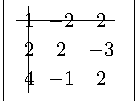
\includegraphics[]{fig/331}
	\end{center}
	Når vi ganger 1 med denne determinanten, har vi funnet det første leddet fra (\ref{3det1}):
	\[ 1\cdot\left|\begin{matrix}
		2 & -3  \\
		-1 & 2
	\end{matrix}\right| \]
	Vi går så over til tallet i første rad og andre kolonne, altså $ -2 $, og finner den tilhørende $ 2\times2 $ determinanten:
	\begin{center}
		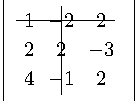
\includegraphics[]{fig/332}
	\end{center}
	Når vi setter et minustegn foran $ -2 $ ganger denne determinanten, har vi funnet andre ledd fra (\ref{3det1}):
	\[ -(-2)\cdot\left|\begin{matrix}
		2 & -3  \\
		4 & 2
	\end{matrix}\right| \]
	Vi avslutter med determinanten vi får ved å utelukke første rad og tredje kolonne:
	\begin{center}
		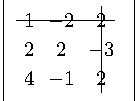
\includegraphics[]{fig/333}
	\end{center}
	Ganger vi denne med tallet som står i både raden og kolonnen som er utelatt, altså 2, får vi siste ledd i (\ref{3det1}):
	\[ 2\cdot\left|\begin{matrix}
		2 & 2  \\
		4 & -1
	\end{matrix}\right| \]
	Vi har nå funnet alle ledd vi trenger og kan da skrive
	\footnotesize
	\alg{
		\det(\vec{a}, \vec{b}, \vec{c}) &= 1\cdot\left|\begin{matrix}
			2 & -3  \\
			-1 & 2
		\end{matrix}\right|-(-2)\cdot\left|\begin{matrix}
			2 & -3  \\
			4 & 2
		\end{matrix}\right|+2\cdot\left|\begin{matrix}
			2 & 2  \\
			4 & -1
		\end{matrix}\right| \\
		&= 2\cdot2-(-3)\cdot(-1)+ 2(2\cdot2-(-3)\cdot4)+ 2(2\cdot(-1)-2\cdot4) \\
		&= 13
	}\vs
}
\section{Vektorproduktet}\index{vektorprodukt}
Vi har sett hvordan vi ved skalarproduktet kan sjekke om to vektorer $ \vec{u} $ og $ \vec{v} $ står normalt på hverandre, men ofte kan vi isteden være interessert i å finne en vektor som står normalt på begge disse. En slik vektor får vi ved \outl{vektorproduktet} av $ \vec{u} $ og $ \vec{v} $, som vi skriver som $ {\vec{u}\times\vec{v}} $.\regv

\reg[\vekpro \label{vekpro}]{
	Vektorpruduktet av vektorene $  {\vec{u}=[a, b, c]} $ og $ {\vec{v}=[d, e, f]} $ er gitt som
	\begin{equation}
		\vec{u}\times\vec{v}=[bf-ce, -(af-cd), ae-bd] \label{vekproeq}
	\end{equation}
	Eventuelt kan man skrive
	\begin{equation}
		\vec{u}\times\vec{v} = \left|\begin{matrix}
			\vec{e}_x & \vec{e}_y & \vec{e}_z \\
			a & b & c \\
			d & e & f
		\end{matrix}\right| \label{vp1}
	\end{equation}
	hvor $ \vec{e}_x=[1, 0, 0], \vec{e}_y=[0, 1, 0] $ og $ \vec{e}_z=[0, 0, 1] $.\vsk
	
	Videre har vi at\footnote{Kryssprodukt må regnes ut før skalarprodukt.}\vs
	\begin{align}
		&\vec{u}\times\vec{v}\cdot\vec{u}=0 \\
		&\vec{u}\times\vec{v}\cdot\vec{v} =0 \\
		&|\vec{u}\times\vec{v}|=|\vec{u}||\vec{v}|\sin \angle(\vec{u}, \vec{v}) \label{vekplen}
	\end{align}\vs\vs
} \vsk
\spr{
Et vektorprodukt kalles også et \outl{kryssprodukt}\index{kryssprodukt}.
} \vsk

\info{\note}{
For skalarproduktet får vi en skalar (et tall), mens vi for vektorproduktet får en vektor. Det er derfor veldig viktig å skille symbolet $ \cdot $ fra $ \times $.
}
\newpage
\eks{
	Gitt vektorene $ {\vec{a}=[-3, 2, 3]} $ og $ {\vec{b}=[2, -2, 1]} $.\os
	\textbf{a)} Finn $ \vec{a}\times\vec{b} $.\os
	\textbf{b)} Vis at vektoren du fant i a) står normalt på både $ \vec{a} $ og $ \vec{b} $. 
	
	\sv
	\textbf{a)} Vi bruker uttrykket fra (\ref{vp1}),	og regner ut følgende $ {3\times3} $ determinant:
	\[ \vec{a}\times\vec{b} =\left|\begin{matrix}
	\vec{e}_x & \vec{e}_y & \vec{e}_z \\
	-3 & 2 & 3 \\
	2 & -2 & 1
	\end{matrix}\right|  \]
	Vi får da at (se gjerne tilbake til eksempelet på side \pageref{eks33})
	\small
	\alg{
		\vec{a}\times\vec{b}&=\vec{e}_x\left|\begin{matrix}
			2 & 3 \\
			-2 & -1
		\end{matrix}\right|-\vec{e}_y\left|\begin{matrix}
			-3 & 3 \\
			2 & 1
		\end{matrix}\right|+\vec{e}_z\left|\begin{matrix}
			-3 & 2 \\
			2 & -2
		\end{matrix}\right|  \\
		&= \vec{e}_x(2\cdot1-3\cdot(-2))-\vec{e}_y(-3\cdot1-3\cdot2)+\vec{e}_z(-3\cdot (-2)-2\cdot2) \\
		&= 8\vec{e}_x+9\vec{e}_y+2\vec{e}_z \\
		&= [8, 9, 2]	
	}
\textbf{b)} To vektorer står normalt på hverandre dersom skalarproduktet av dem er 0:\vs \alg{
&[8, 9, 2]\cdot[-3,2,3]=-24+18+6=0 \os
&[8, 9, 2]\cdot[2,-2,1]=16-18+2=0
}
\vs
} \vsk
\reg[Regneregler for vektorproduktet]{
	For vektorene $ \vec{u}, \vec{v} $ og $ \vec{w} $ og en konstant $ t $ har vi at
	\begin{align}
		\vec{u}\times\vec{v} &= -\vec{v}\times\vec{u} \\
		\vec{u}\times{(t\vec{v})} &= t(\vec{u}\times\vec{v}) \\
		\vec{u}\times(\vec{v}+\vec{w})&=\vec{u}\times\vec{v}+\vec{u}\times\vec{w}\\
		\vec{u}\times\vec{v}\cdot\vec{w}&= \vec{w}\times\vec{u}\cdot\vec{v} \label{ukryvpriw}
	\end{align}\vs
}
\newpage
\subsection{Vektorprodukt som areal og volum}\index{vektorprodukt!som areal og volum}
En anvendelse av vektorproduktet (og skalarproduktet) er å finne arealet og volumet av noen geometriske former som kan sies å være \textsl{utspent}\index{utspent!geometrisk figur} av vektorer. Med dette mener vi at to eller tre vektorer som starter i samme utgangspunkt, utgjør grunnlaget for en trekant, et parallellogram, et \outl{parallellepiped}, en pyramide eller et \outl{tetraeder}.
\begin{figure}
	\centering
	\subfloat[Trekant]{\includegraphics[]{\figp{trk}}}\qquad
	\subfloat[Parallellogram]{\includegraphics[]{\figp{parll}}}\\
	\subfloat[Parallellepiped]{\includegraphics[]{\figp{par}}}
	\subfloat[Pyramide]{\includegraphics[]{\figp{pyram}}}\quad
	\subfloat[Tetraeder]{\includegraphics[]{\figp{tetra}}}
	\captionof{figure}{Geometriske former utspent av vektorene $ \vec{u} $, $ \vec{v} $ og $ \vec{w} $.}\index{parallellogram}\index{trekant}\index{parallellepiped}\index{pyramide}\index{tetreaeder}
\end{figure}

\reg[\vekproarvol \label{vekproarvol}]{
	Arealet $ A $ av et parallellogram utspent av vektorene $ \vec{u} $ og $ \vec{v} $ er gitt som
	\nreq{A = |\vec{u}\times\vec{v}| \label{vekpar} }
	%	\includegraphics[scale=1]{\asym{parll}}
	Arealet $ A $ av en trekant utspent av vektorene $ \vec{u} $ og $ \vec{v} $ er gitt som
	\nreq{A = \frac{1}{2}|\vec{u}\times\vec{v}|\label{vektre}}
	Volumet $ V $ av parallellepipedet utspent av vektorene $ \vec{u}$, $ \vec{v} $ og $ \vec{w} $ er gitt som
	\nreq{V = \left|\vec{u}\times\vec{v}\cdot\vec{w}\,\right|}
	%\includegraphics[scale=1]{\asym{par}}
	Volumet $ V $ av pyramiden utspent av vektorene $ \vec{u}$, $ \vec{v} $ og $ \vec{w} $ er gitt som
	\nreq{V = \frac{1}{3}|\vec{u}\times\vec{v}\cdot\vec{w}\,|\label{volavpyr} }
	%\includegraphics[scale=1]{\asym{pyram}}
	Volumet $ V $ til tetraedet utspent av vektorene $ \vec{u}$, $ \vec{v} $ og $ \vec{w} $ er gitt som			
	\nreq{ V = \frac{1}{6}|\vec{u}\times\vec{v}\cdot\vec{w}\,|}\vs
	%\includegraphics[scale=1]{\asym{tetra}}	
}

\newpage
\tsec{Forklaringer}
\fork{\ref{parvek} \parvek}{
Ligning \eqref{vekpar} forteller oss at $ {|\vec{u}\times\vec{v}|} $ tilsvarer arealet av parallellogramet utspent av $ \vec{u} $ og $ \vec{v} $. Dette arealet kan bare ha verdien 0 hvis $ \vec{u} $ og $ \vec{v} $ er parallelle, og den eneste vektoren med lengde 0 er nullvektoren $ [0, 0, 0] $. Kombinerer vi dette kravet med \eqref{vekpro}, får vi at
\[ [y_1z_2-z_1y_2, -(x_1z_2-z_1x_2), x_1y_2-y_1x_2]=[0, 0, 0] \]
Uttrykket over gir oss tre ligninger
\alg{
	y_1z_2-z_1y_2&= 0	 \os
	x_1z_2-z_1x_2&= 0 \os
	x_1y_2-y_1x_2&=0
}
som vi kan omskrive til
\alg{
	\frac{y_1}{y_2}&=\frac{z_1}{z_2} &	
	\frac{x_1}{x_2}&=\frac{z_1}{z_2} &
	\frac{x_1}{x_2}&=\frac{y_1}{y_2}
}
Til slutt kan vi samle alle tre til én ligning:
\[\frac{x_1}{x_2}= \frac{y_1}{y_2}=\frac{z_1}{z_2} \]
} \vsk

\fork{\ref{vekpro} \vekpro}{
Hensikten med vektorproduktet er å innføre en regneoperasjon som gir oss en vektor $  {\vec{w}=[x, y, z]} $ som står normalt på to andre vektorer $ {\vec{u}=[a, b, c]} $ og $ {\vec{v}=[d, e, f]} $. For at dette skal være sant, vet vi av (\ref{vnkr}) at \vs
\begin{align}
	\vec{u}\cdot\vec{w}&=0 \nonumber \\ 
	ax+by+cz &=0 \nonumber\\
	ax+by &= -cz\label{vktp2}\\
	& \nonumber \\
	\vec{v}\cdot\vec{w}&=0 \nonumber \\ 
	dx+ey+fz&=0  \nonumber \\
	dx+ey&=-fz\label{vktp5}
\end{align}
Vi har altså to forskjellige ligninger som kan hjelpe oss med å finne de tre ukjente størrelsene $ x, y $ og $ z$. Dette kalles at man har en ligning med \textit{én fri variabel}. Hvis vi velger $ z $ som fri variabel betyr dette kort fortalt at vi kan finne et uttrykk for $ x $ og $ y $ som vil oppfylle (\ref{vktp2}) og (\ref{vktp5}) for et hvilket som helst valg av $ z $. \vsk

Vi starter med å finne et uttrykk for $ x $. Først multipliserer vi (\ref{vktp5}) med $ \frac{b}{e} $, og subtraherer deretter venstre- og høyresiden fra denne ligningen med henholdsvis venstre- og høyresiden fra ligning (\ref{vktp2}):
\alg{
	ax+by -\left(\frac{bdx}{e}+by\right)&= -cz-\left(-\frac{bfz}{e}\right) \\
	ax - \frac{bdx}{e}&=-cz-\left(-\frac{bfz}{e}\right)
}
Hvis vi videre multipliserer med $ e $, og deretter antar at $ ae-bd\neq0 $, får vi at
\begin{align}
	aex -bdx &= bfz-cez \nonumber\\
	(ae-bd)x &= (bf-ce)z\nonumber \\
	x &= \frac{bf-ce}{ae-bd}z \label{x}
\end{align}
Med omtrent samme framgangsmåte og identisk antakelse finner vi et uttrykk for $ y $:
\begin{align}
	ax+by -\left(ax+\frac{aey}{d}\right)&= -cz-\left(-\frac{afz}{d}\right) \nonumber\\
	(bd-ae)y &= (af-cd)z \nonumber\\
	y &= \frac{af-cd}{bd-ae}z \label{y}
\end{align}
Som nevnt kan $ z $ velges fritt, og vi ser av (\ref{x}) og (\ref{y}) at valget $ {z=ae-bd} $ gir oss følgende fine uttrykk:
\alg{
	x &= bf-ce \\
	y &= -(af-cd) \\
	z &= ae-bd
} 
Dette samsvarer med (\ref{vekpro}). \vsk

For å komme fram til likhetene over har vi antatt at $ {z=ae-bd\neq 0} $, men det er fristende å sjekke om uttrykkene vi nettopp har funnet oppfyller (\ref{vktp2}) og (\ref{vktp5}) også når ${ z=ae-bd=0} $:
\alg{ax+by &=0 \\
	a(bf-ce)+-b(af-cd) &= 0 \\
	-(ae-bd)c &= 0\\
	0 &= 0 \\
	& \\
	dx + ey &= 0 \\
	d(bf-ce)-e(af-cd)&=0 \\
	-(ae-db)f &= 0 \\
	0 &= 0 
}
Med $ z $ som fri variabel er altså (\ref{vktp2}) og (\ref{vktp5})  oppfylt for alle ${ z=ae-bd} $, dermed har vi funnet et uttrykk som alltid vil gi oss en vektor $ \vec{w} $ som er ortogonal med både $ \vec{u} $ og $ \vec{v} $. \vsk

Så lenge man bruker uttrykkene fra \eqref{x} og \eqref{y}, vil $ \vec{w} $ være parallell med vektoren gitt ved (\ref{vekpro}), uansett valg av $ z $. I tillegg kan vi få uttrykket fra (\ref{vekpro}) også om vi velger $ x $ eller $ y $ som fri variabel (det får bli opp til leseren å konstatere disse to påstandene).\label{allekrypropar} Av dette kan vi konkludere med at alle vektorer som står ortogonalt på både $ \vec{u} $ og $ \vec{v} $ er parallelle med vektoren gitt ved (\ref{vekpro}). \vsk

\textbf{Lengden til vektorproduktet}\os
For å komme fram til det vi ønsker, skal vi benytte oss av \outl{Lagranges identitet}\footnote{Den spesielt interesserte finner utledningen for identieten i \refved{lagrange}}\index{Lagranges identitet.}. Denne sier at vi for to vektorer
$ \vec{v} $ og $ \vec{u} $ har at
\[\phantom{testingcloservl} |\vec{v}\times\vec{u}|^2=|\vec{v}|^2|\vec{u}|^2-(\vec{v}\cdot\vec{u}\,)^2 \tag{Lagranges identitet}\]
Ved å anvende \eqref{skal2} og \eqref{1} kan vi skrive 
\alg{
	|\vec{v}\times\vec{u}|^2&=|\vec{v}|^2|\vec{u}|^2-|\vec{v}|^2|\vec{u}|^2\cos^2 \theta \\
	|\vec{v}\times\vec{u}|^2&= |\vec{v}|^2|\vec{u}|^2(1-\cos^2 \theta) \\
	|\vec{v}\times\vec{u}| &= |\vec{v}||\vec{u}|\sin \theta 	
}
}
\begin{comment}
svar på gruble
	\subsection*{\boldmath $ 2\times2 $ determinanten som areal}
	\subimport{fig/}{det}
	La oss ta utgangspunkt i et parallellogram utspent av to vektorer $ \vec{u}=[a, b] $ og $ \vec{v}=[c, d] $ med en vinkel $ \theta \leq 90^\circ $ mellom seg, som skissert i \fref{det}. Fra klassisk arealregning og trigonometri vet vi at arealet $ A $ av parallallogrammet er:
	\[ A = |\vec{v}||\vec{u}|\sin \theta  \]
	Ved hjelp av identieten fra ref?? kan vi omskrive dette til:
	\begin{equation}
	A = |\vec{v}||\vec{u}|\cos (90^\circ -\theta) \label{ardet}
	\end{equation}
	Vi kan altså tolke $ A $ som skalarproduktet av $ \vec{u} $ og en vektor $ \vec{w} $ med samme lengde som $ \vec{v} $, men en retning slik at $ \angle(\vec{u}, \vec{w})=(90^\circ-\theta) $. Dette medfører at $\angle (\vec{v},\vec{w} )=90^\circ $, og da blir $ \vec{w}\cdot\vec{v}=0 $. Derfor må vi ha at:
	\[ \vec{w}=[-d, c] \quad\vee\quad \vec{w}=[d, -c] \] 
	Bare én av disse gir oss den ønskede retningen som fører oss tilbake til (\ref{ardet}), men vi merker oss følgende:
	\[\cos \angle(\vec{u}, \vec{w}) = \frac{bc-ad}{|\vec{u}||\vec{w}|} \quad \vee \quad \cos \angle(\vec{u}, \vec{w}) = -\frac{bc-ad}{|\vec{u}||\vec{w}|}\]
	De to mulige cosinusverdiene har altså eksakt samme tallverdi. Tar vi nå absoluttverdien av $ \vec{u}\cdot\vec{w} $, kan vi derfor være sikre på at vi har det samme uttrykket som i (\ref{ardet}):
	\alg{
	A &= |\vec{v}||\vec{u}|\cos (90^\circ -\theta)\\
	&= |\vec{u}\cdot\vec{w}| \\
	&= |ad-bc|}
	For $ \theta>90^\circ $ kan vi gå fram på akkurat samme måten som vi nå har gjort, og vi regner oss dermed som ferdige med forklaringen.
\end{comment}

\fork{\ref{vekproarvol} \vekproarvol}{ \vsb
\figc{parlb}{Parallellogram med grunnlinje $ |\vec{u}| $ og høyde $ |\vec{v}|\sin \theta $.}
Arealet av et paralellogram er gitt som grunnlinja ganger høyden. For et parallellogram utspent av vektorene $ \vec{u} $ og $ \vec{v} $, tilsvarer dette produktet $ |\vec{u}||\vec{v}|\sin \theta $, som er det samme som lengden $ |\vec{u}\times\vec{v}| $. Arealet av trekanten utspent av $ \vec u $ og $ \vec{v} $ er halvparten av arealet av parallellogrammet.
\subsection*{Vektorproduktet som volum \label{vekprsomvolforkl}}
\figc{par}{\label{vopar3}}
Volumet $ V $ av et parallellepidet tilsvarer grunnflaten $ A $ ganger høyden $ h $:
\begin{equation}
	V = Ah \label{vopar0}
\end{equation}
\begin{figure}
	\centering
	\includegraphics[]{\figp{vopar}}\qquad
	\includegraphics[]{\figp{voparb}}
	\captionof{figure}{\label{vopar}}	
\end{figure}
I \fref{vopar3} er grunnflaten $ A $ utspent av vektorene $ \vec{v} $ og $ \vec{v} $, og vi vet fra (\ref{vekpar}) at
\begin{equation}
	A = |\vec{u}\times\vec{v}|  \label{vopar1}
\end{equation}
La $ \theta $ være vinkelen mellom  $ \vec{u}\times\vec{v} $ og $ \vec{w} $. Hvis $ {90^\circ\geq\theta\geq0} $, får vi en figur som skissert i \fref[a]{vopar}. Da er høyden $ h $ gitt som
\[ h = |\vec{w}\,|\cos \theta \]
Er derimot $ {180^\circ\geq\theta>90^\circ} $, får vi en figur som skissert i \fref[b]{vopar}. Da er
\[ h = -|\vec{w}\,|\cos \theta \]
For alle $ \theta\in[0^\circ, 180^\circ] $ kan vi derfor skrive
\begin{equation}
	h = \big| |\vec{w}\,|\cos \theta \big| \label{vopar2}
\end{equation}
Av \eqref{skal2}, \eqref{vopar0}, \eqref{vopar1} og \eqref{vopar2}, og  har vi derfor at
\alg{
	\big|\vec{u}\times\vec{v}\cdot\vec{w}\,\big|&= \big||\vec{u}\times\vec{v}||\vec{w}\,|\cos \theta\big|\\
	&=Ah \\
	&= V	
}
Av klassisk geometri har vi videre at
\begin{itemize}
	\item volumet av pyramiden utspent av $ \vec{u} $ og $ \vec{v} $ er $ \frac{1}{3} $ av volumet av parallellepipedet.
	\item volumet av tetraedet utspent av $ \vec{u} $ og $ \vec{v} $ er $ \frac{1}{6} $ av volumet av parallellepipedet.
\end{itemize} 
}

\end{document}